\chapter{Network Architecture}
\label{ch:architecture}

This project's target network is a new experimental-production network located in Barcelona. It has been deployed in order to prove its stability, robustness and feasibility to replicate it in other Barcelona's locations with similar topologies. This network's main particularity is that it merges different network topologies requiring the use of Exterior Gateway Protocols (BGP) together with Internal Gateway Protocols (BMX6) in order be able to share routes between different BGP ends (named \textit{E} and \textit{F} in the figure \ref{fig:tarnet}) going through a Mesh Network. The following information has been extracted from the report "Integració entre BMX6 i BGP en dispositius basats en LEDE" \cite{bgpbmx6} (in Catalan).

As shown in the figure \ref{fig:tarnet}, network's elements are:
\begin{itemize}
    \item \textbf{Infrastructure Super Node 1} (ISN1): BGP Supernode connected to the BGP network (Guifi.net, section 1) via wireless and to the MXN1 Router through Ethernet.     
    \item \textbf{Mesh eXchange Node 1} (MXN1): LEDE/OpenWRT router connected via Ethernet to the ISN1 and to the antenna (or an Ethernet port) providing access to the Mesh Network. This frontier node provides BGP to BMX6 route-sharing capabilities using Bird Daemon.
    \item \textbf{Mesh Network}: A number of Nodes connected using BMX6 forming an isle between BGP nodes.
    \item \textbf{Mesh eXchange Node 2} (MXN2): LEDE/OpenWRT router connected via Ethernet to the ISN2 and to the antenna (or an Ethernet port) providing access to the Mesh Network. This frontier node provides BGP to BMX6 route-sharing capabilities using Bird Daemon.
    \item \textbf{Infrastructure Super Node 2} (ISN1): BGP Super Node connected to the BGP network (Guifi.net, section 2) via wireless and to the MXN2 Router through Ethernet.
\end{itemize}


\section{Routing requirements}
Routing requirements to successfully ensure that all routes are shared between both BGP ends are:

\begin{itemize}
    \item Routes must be shared/announced between ISN1 (\textbf{E}) and ISN2 (\textbf{F}).
    \item Mesh Network's Routes (BMX6 - \textbf{C}\&\textbf{D}) must be shared/announced to ISN1 and ISN2 (\textbf{A}\&\textbf{B}). Therefore, shared/announced to Guifi.net network.
    \item ISN1 and ISN2 Routes (BGP - \textbf{A}\&\textbf{B}) must be shared/announced to the Mesh Network (\textbf{C}\&\textbf{D}).
    \item MXN1/2 must configure Bird to use a custom Routing Table that will be shared with BMX6.
    \item MXN1/2 must configure BMX6 to use the \textit{Table} plugin in order to redirect its routes from Kernel's Table to a custom one.
    \item MXN1/2 must configure Bird to set them both as BGP Peers to stablish an iBGP session between them (AS2).
    \item MXN1 must configure Bird to set ISN1 as BGP Peer AS1
    \item MXN2 must configure Bird to set ISN1 as BGP Peer AS3
\end{itemize}

\subsection{Caveats}
There is an important caveat with this network distribution:

Current version of BMX6 is not able to handle the number of announced prefixes that Barcelona's Guifi.net BGP sessions are currently sharing (3.500+). Therefore, in order to be able to handle those received network prefixes, BMX6 will have to start aggregating its routes, which eventually would shut-down the service and leave the node overloaded or even unresponsive.

In order to avoid this disruptive behaviour, Bird Daemon filter scripting capabilities available in MXN1 and MXN2 allow to reduce the geographical scope of the prefixes imported and exported to and from the Barcelon\`{e}s zone (including cities: Badalona, Barcelona, Hospitalet del Llobregat, Sant Adri\`{a} del Besos and Santa Coloma de Gramanet).

\begin{landscape}

\begin{figure}[ht!]
    \centering
    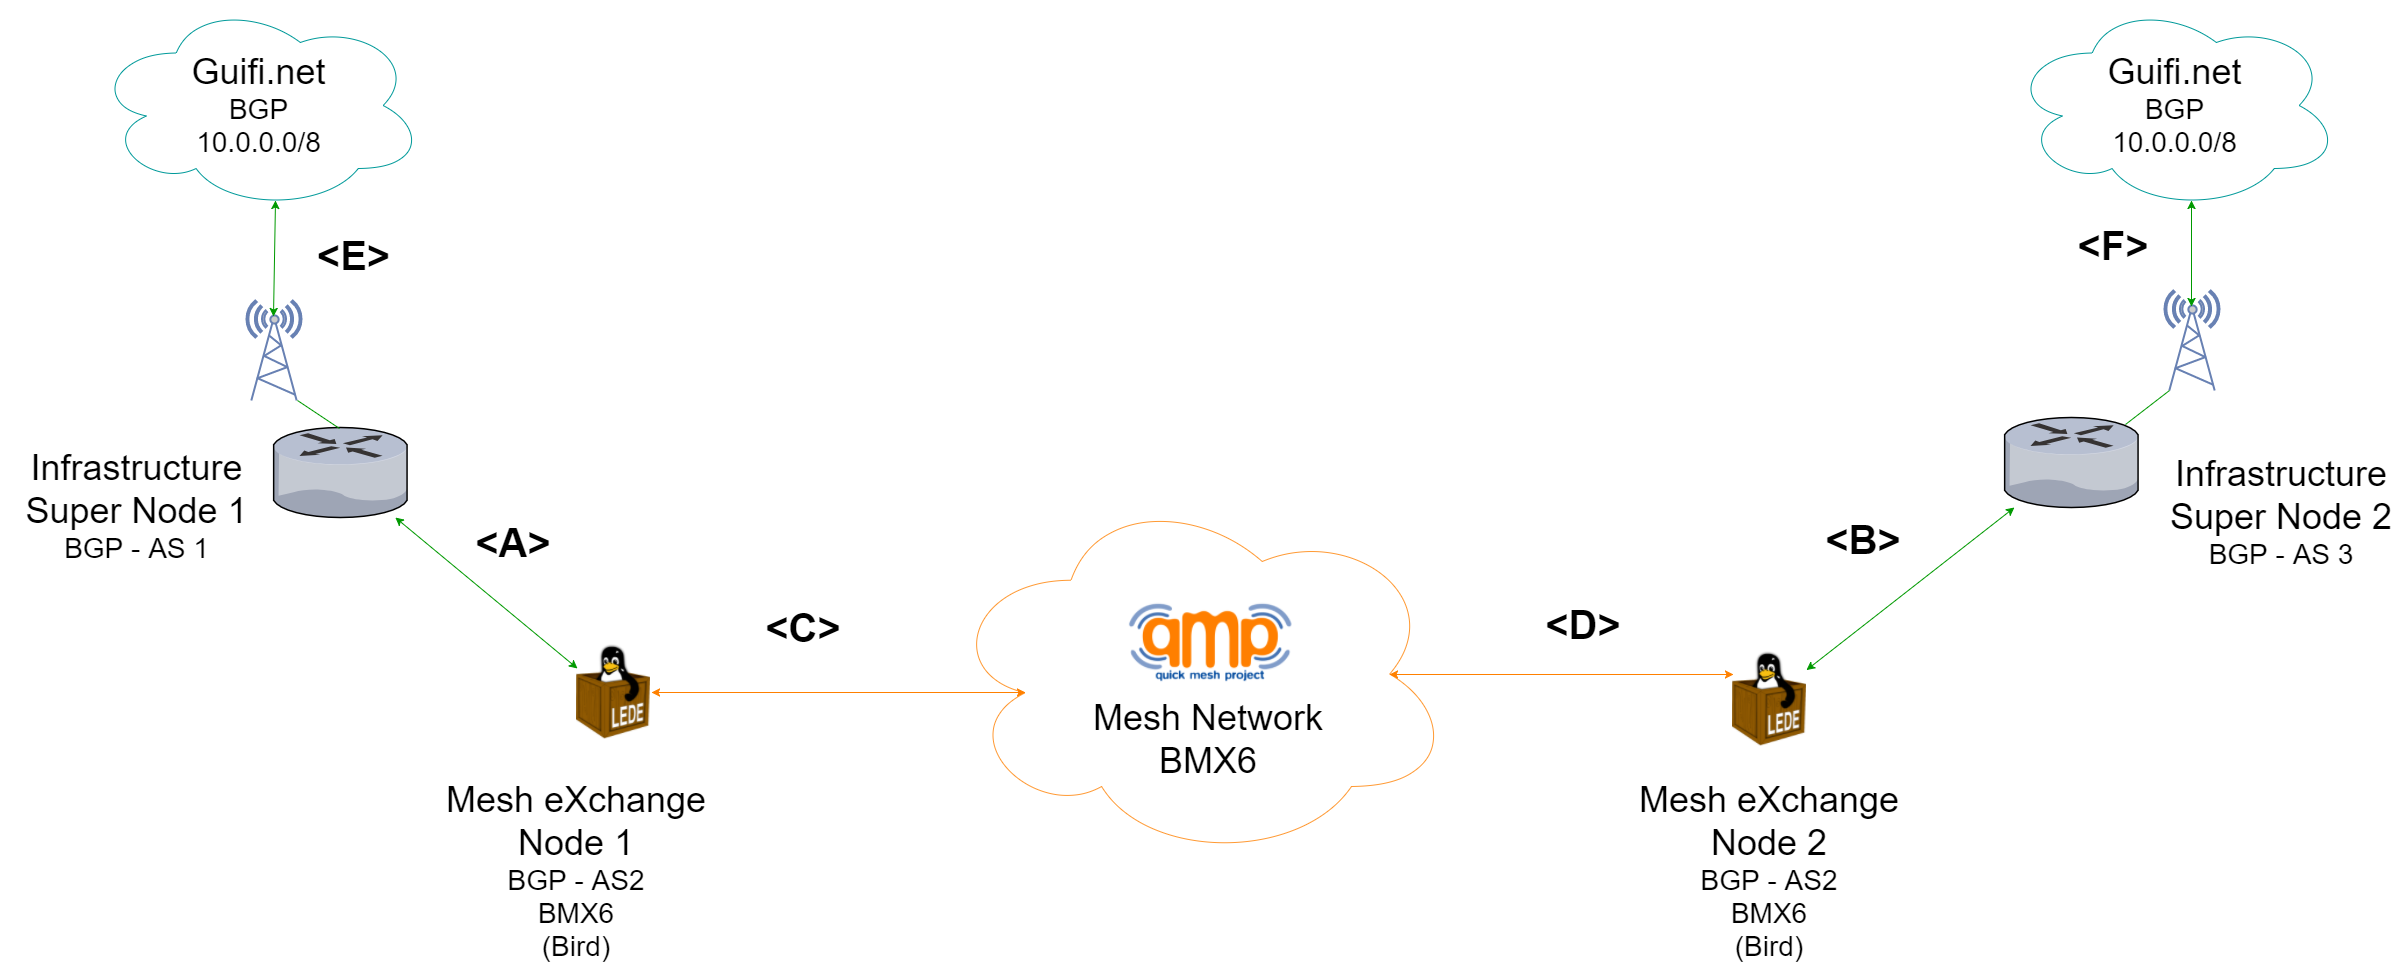
\includegraphics[width=\hsize]{images/targetnet}
    \caption{Production Network targeted in this project}
    \label{fig:tarnet}
\end{figure}
\end{landscape}
\newpage

\section{Testing Scenarios}
Although it has not been possible to test Package's improvements in the target production network as the changes would incur in service disruption for up to 1500+ nodes in the Barcelon\`{e}s Zone, it is foreseen to update target \textit{MXN} Nodes after agreeing it with all the involved parts.

Nevertheless, this Package's improvements have been tested in two different environments connected directly with Guifi.net thanks to Universitat Oberta de Catalunya and V\'{i}ctor's support, who have provided and helped me configuring a number of Virtual Machines, virtual network resources and also agreed permission to get through another university's network, Universitat Pompeu Fabra, in order to connect to a different network section, but still in Barcelona, thus following the same approach of different BGP Peers being able to route and share prefixes: 

\subsubsection{Internal Development Testing}
Package development tests have been done inside UOC's network using a really simple network topology where our target Bird Node VM is connected to Guifi.net using UOC's Infrastructure Node (UOC receives/announces 3000+ BGP Routes). 

\begin{figure}[H]
        \centering
        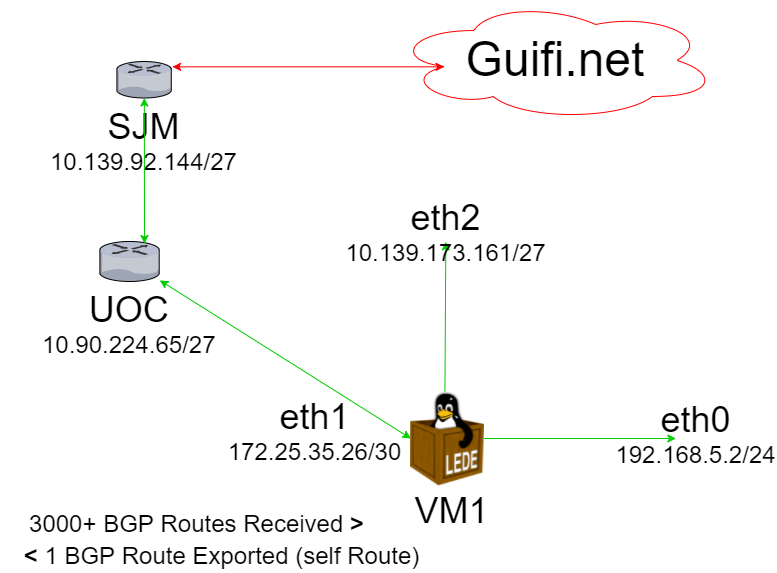
\includegraphics[width=0.8\textwidth]{images/devmin}
        \caption{Minimal test environment.}
        \label{fig:mindev}
	\end{figure}

\subsubsection{Final Package Testing}
As can be seen in the Figure \ref{fig:devnet}, the final testing environment is a virtual mirror of the target network. This environment has been created in order to do the final tests after \textit{releasing} the final version of the Package to test it without the risk of damaging the production network or flooding unwanted routes to Guifi.net. This network section routes to two Infrastructure Super Nodes connected to two geographically-separated Barcelona well-known Universities, being almost, if not exactly, a mirror of what our target network is.

The components provided in order to achieve this network have been:
\begin{itemize}
    \item VPN access to the Guifi Network using UOC's resources.
    \item 4 Virtual Machines using LEDE17.01 Firmware in University's network.
    \item Virtual Bridge to connect the VMs simulating a fully connected Mesh Network.
    \item Network way through two different Barcelona's network sections.
    \begin{itemize}
        \item Virtual Machine 1 connects through UOC's Super Node
        \item Virtual Machine 4 connects through UPF's internal network, to a near Guifi network section.
        \item Both Infrastructure SuperNodes are importing all their routes to our network
        \item UPF's SuperNode throughput has been limited to avoid disruption in their internal network.
        \begin{itemize}
            \item Connection through UPF's internal network using a IPIP Tunnel: IP inside IP encapsulates IP Addresses and their datagram inside other IP Addresses.
            \item We have agreed to do this testing in a limited time-frame to avoid disruption in their services as we are sharing routes between Guifi.net-UOC-UPF-Guifi.net.
        \end{itemize}
    \end{itemize}
\end{itemize}

\subsubsection{Testing environment elements}
\begin{itemize}
    \item \textbf{SJM}: Guifi.net Node  \href{https://guifi.net/en/node/20262/}{BCNSantJoanDeMalta51}. Infrastructure Node with 6 Point-to-Point connections to other Super Nodes. As we have no control on this node, we will consider that it is importing and exporting any received route to/from Guifi.net.
    \item \textbf{UOC}: Guifi.net Node \href{https://guifi.net/en/node/63255}{BCNRamblaPobleNou156}. Infrastructure Node located in the Universitat Oberta de Catalunya and connected to the Super Node BCNSantJoanDeMalta51. This node is shown as AS1.
    \item \textbf{VM1}: KVM\footnote{KVM: Kernel-based Virtual Machine.} Virtual Machine acting as Frontier Node (MXN1). This node is configured with Bird Daemon (BGP AS2) and BMX6 in order to connect to its BGP neighbour AS1 (ISN1), to its iBGP Peer AS2 (MXN2) and to the BMX6 Mesh network.
    \item \textbf{VM2 \& VM3}: KVM Virtual Machines acting as plain Mesh nodes.
    \item \textbf{VM4}: KVM Virtual Machine acting as Frontier Node (MXN2). This node is configured with Bird Daemon (BGP AS2) and BMX6. It connects to its BGP neighbour AS3 (ISN2) over a GRE Tunnel configured in UPF's internal network, also to its iBGP Peer AS2 (MXN2) and to the BMX6 Mesh network.
    \item \textbf{UPF}: Guifi.net Node \href{https://guifi.net/en/node/56604}{BCNUPFPobleNou}. Infrastructure Node located in the Universitat Pompeu Fabra and reached through UPF's internal network. Therefore, VM4 connects using an internal IP Address supplied by UPF's administrators. This node is shown as AS3.
\end{itemize}


\begin{landscape}
\begin{figure}[ht!]
    \centering
    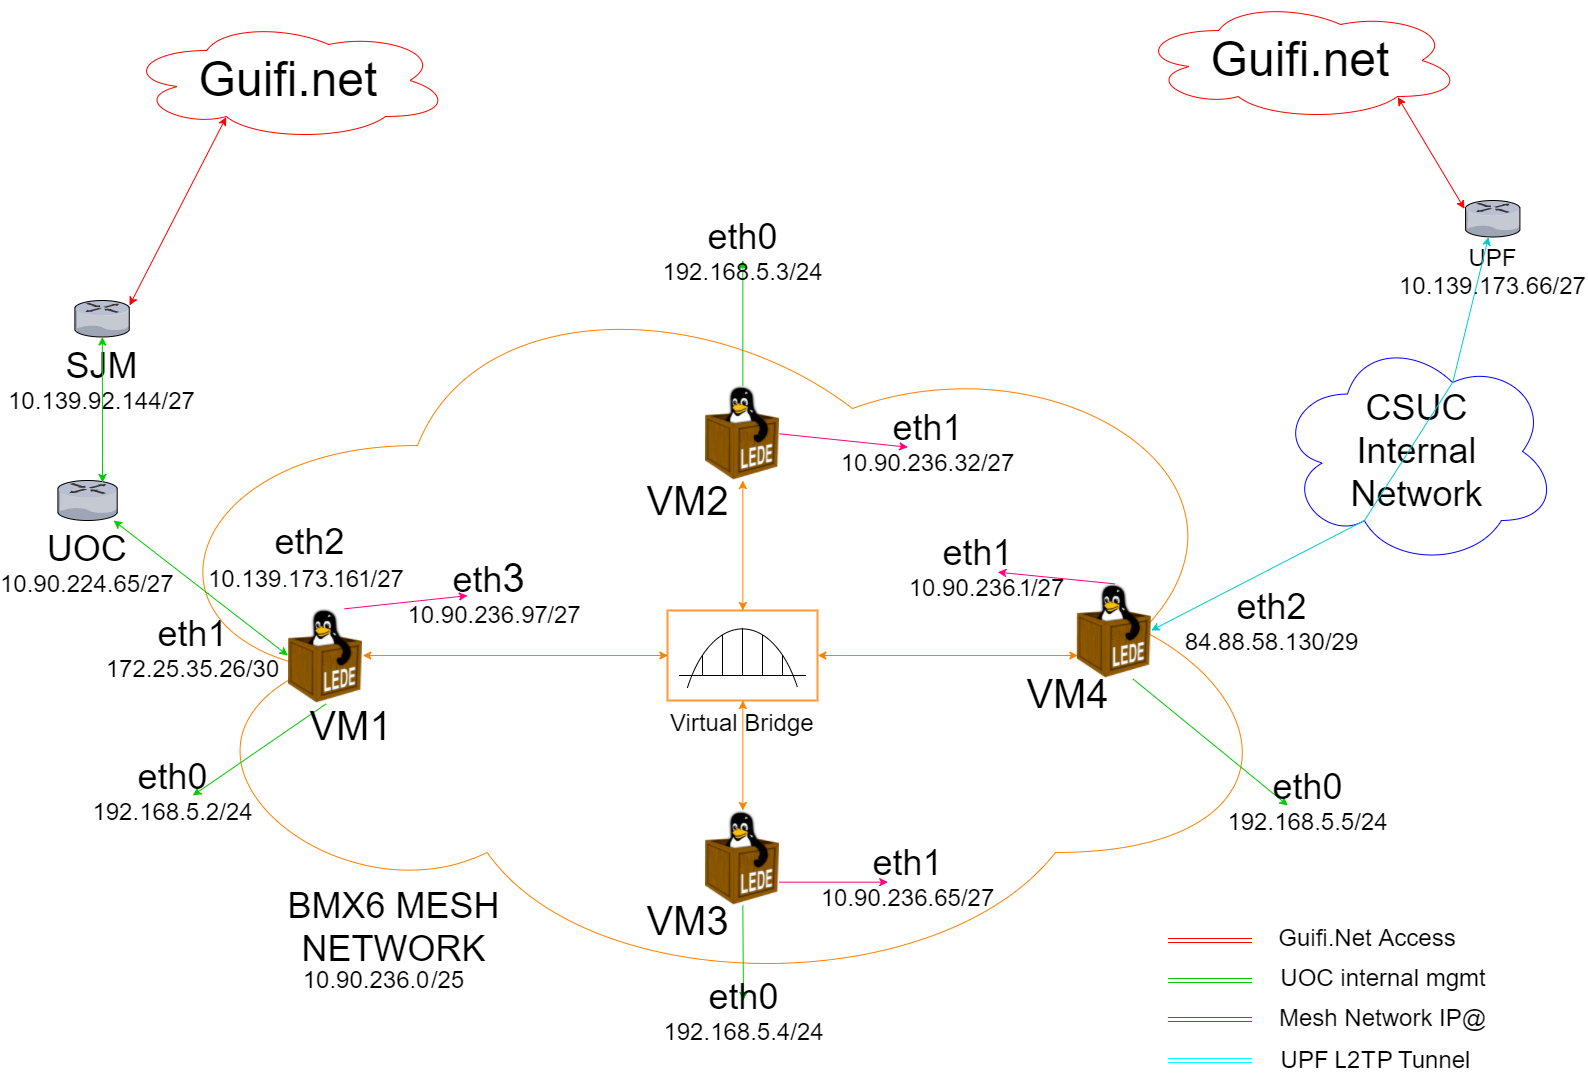
\includegraphics[width=\hsize]{images/devnetfull}
    \caption{Development Network simulating production's environment}
    \label{fig:devnet}
\end{figure}
\end{landscape}
\newpage

